\documentclass[a4paper,12pt]{article}
\usepackage[english,ukrainian,russian]{babel}
\linespread{1}
\usepackage{ucs}
\usepackage[utf8]{inputenc}
\usepackage[T2A]{fontenc}
\usepackage[paper=portrait,pagesize]{typearea}
\usepackage{amsmath}
\usepackage{bigints}
\usepackage{amsfonts}
\usepackage{graphicx}
\usepackage{amssymb}
\usepackage{cancel}
\usepackage{gensymb}
\usepackage{multirow}
\usepackage{rotate} 
\usepackage{pdflscape}
\usepackage{bigstrut}
\usepackage[pageanchor]{hyperref}
\usepackage{chngpage}
\usepackage{fancybox,fancyhdr}
\newcommand\tab[1][1cm]{\hspace*{#1}}
\newcommand{\RomanNumeralCaps}[1]{\MakeUppercase{\romannumeral #1}}
\usepackage[left=20mm, top=20mm, right=15mm, bottom=15mm, nofoot]{geometry}

\usepackage{verbatim}
\usepackage{enumerate}
\usepackage{listings}
\usepackage{xcolor}

\definecolor{codegreen}{rgb}{0,0.6,0}
\definecolor{codegray}{rgb}{0.5,0.5,0.5}
\definecolor{codepurple}{rgb}{0.58,0,0.82}
\definecolor{backcolour}{rgb}{0.95,0.95,0.92}

\lstdefinestyle{mystyle}{
	backgroundcolor=\color{backcolour},   
	commentstyle=\color{codegreen},
	keywordstyle=\color{blue},
	numberstyle=\tiny\color{codegray},
	stringstyle=\color{red},
	basicstyle=\ttfamily\footnotesize,
	breakatwhitespace=false,         
	breaklines=true,                 
	captionpos=b,                    
	keepspaces=true,                 
	numbers=none,                    
	numbersep=5pt,                  
	showspaces=false,                
	showstringspaces=false,
	showtabs=false,                  
	tabsize=4,
	frame=shadowbox
}

\lstset{style=mystyle}

\begin{document}
    \pagestyle{fancy}
    \fancyhead{}
    \fancyhead[R]{ФІ-12 Завалій Олександр}
    \begin{center}
        \large{\textbf{Міністерство освіти і науки України\\
                Національний технічний університет України\\
                «Київський політехнічний інститут імені Ігоря Сікорського»\\
                Навчально-науковий Фізико-технічний інститут}}\\
        \hfill \break \hfill \break \hfill\break \hfill \break \hfill \break \hfill \break \hfill \break
        \hfill \break \hfill \break \hfill \break
        \begin{center}
            \normalsize{\textbf{Архітектура комп'ютерних систем\\
            Комп’ютерний практикум\\
            Робота №1}}
        \end{center}
    \end{center}
    \hfill \break \hfill \break \hfill \break \hfill \break \hfill \break \hfill \break \hfill \break
    \hfill \break \hfill \break \hfill \break \hfill \break 
    \begin{flushright}
        \large{ \hspace{35pt} Виконав:\\
            студент групи ФI-12\\
            Завалій Олександр\\} 
        \large{ \hspace{35pt} Перевірив:\\
        Козленко О.В.} 
    \end{flushright}
    \hfill \break \hfill \break \hfill \break \hfill \break \hfill \break \hfill \break \hfill \break
    \hfill \break
    \begin{center} \textbf{Київ-2024} \end{center}
    \thispagestyle{empty}

\newpage
    \begin{center}
        \section*{\bfseries{Робота №1.\\
        Порівняння програми, написаної на мові 
        високого рівня з її компільованим виглядом
    }}
    \end{center}
    \textbf{Мета:} \\
    \hangindent=1.5cm 
    \hangafter=+1 \noindent
    Ознайомитися з основам дизасемблінгу та з представленням основних
    базових арифметичних дій, структур умови та переходу, з представленням
    локальних та глобальних змінних, циклів, викликів функцій, визначення масиву у
    мові асемблер в архітектурі ІА-32. \\
    \begin{center}
        \Large{Варіант №4}
    \end{center}
    Зміст індивідуального завдання:
    \begin{enumerate}
        \item Базові арифметичні дії (віднімання, множення), значення елементів
        визначає користувач
        \item if стейтмент рядок
        \item Switch на 3 пунктів
        \item Глобальними та локальними змінними
        \item Циклом for
        \item Викликом функції, яку ви створили
        \item Массивом з такими елементами: 34,56,32,12
    \end{enumerate}

\newpage
    \begin{center}
        \Large{Code}
    \end{center}
    \begin{lstlisting}[language=C++]
#include <iostream>
using namespace std;
int a, b, num;
void task_4();

void task_1(){
    cout<<"---Task 1--- \nEnter numbers A&B:\n";
    cin>>a>>b;
    cout<<"a - b = "<<a-b<<"\na * b = "<<a*b<<"\n";
}
void task_2(){
    cout<<"\n---Task 2--- \nEnter a number:\n";
    cin>>a;
    if (a % 2 == 0){
        cout<<"This number is even\n"; } else { cout<<"This number is odd\n"; }
}
void task_3(){
    cout<<"\n---Task 3--- \nEnter the task number\n";
    cin>>num;
    switch (num) {
        case 1:
            task_1();
            break;
        case 2:
            task_2();
            break;
        case 3:
            task_4();
            break;}
}
void task_4(){
    cout<<"\n---Task 4--- \nGlobal variables A,B and num have the following values:\n";
    cout<<"A: "<<a<<"\nB: "<<b<<"\nnum: "<<num<<"\n";
}
void task_5(){
    int c;
    cout<<"\n ---Task 5--- \nEnter a number:\n";
    cin>>c;
    for(int i=1; i<c+1; i++){
        cout<<i;}
    cout<<endl;
}
void task_7(){
    cout<<"\n---Task 7---\n";
    int arr[5] = {34,56,32,12};
    cout<< arr[3];
}

int main() {    
    task_1();
    task_2();
    task_3();
    task_4();
    task_5();
    task_7();
    return 0;
}
    \end{lstlisting}

\newpage
    \begin{center}
        \Large{Task \RomanNumeralCaps{1}}
    \end{center}
    \begin{figure}[h!]
        \begin{minipage}[h]{1\linewidth}
            \centering
            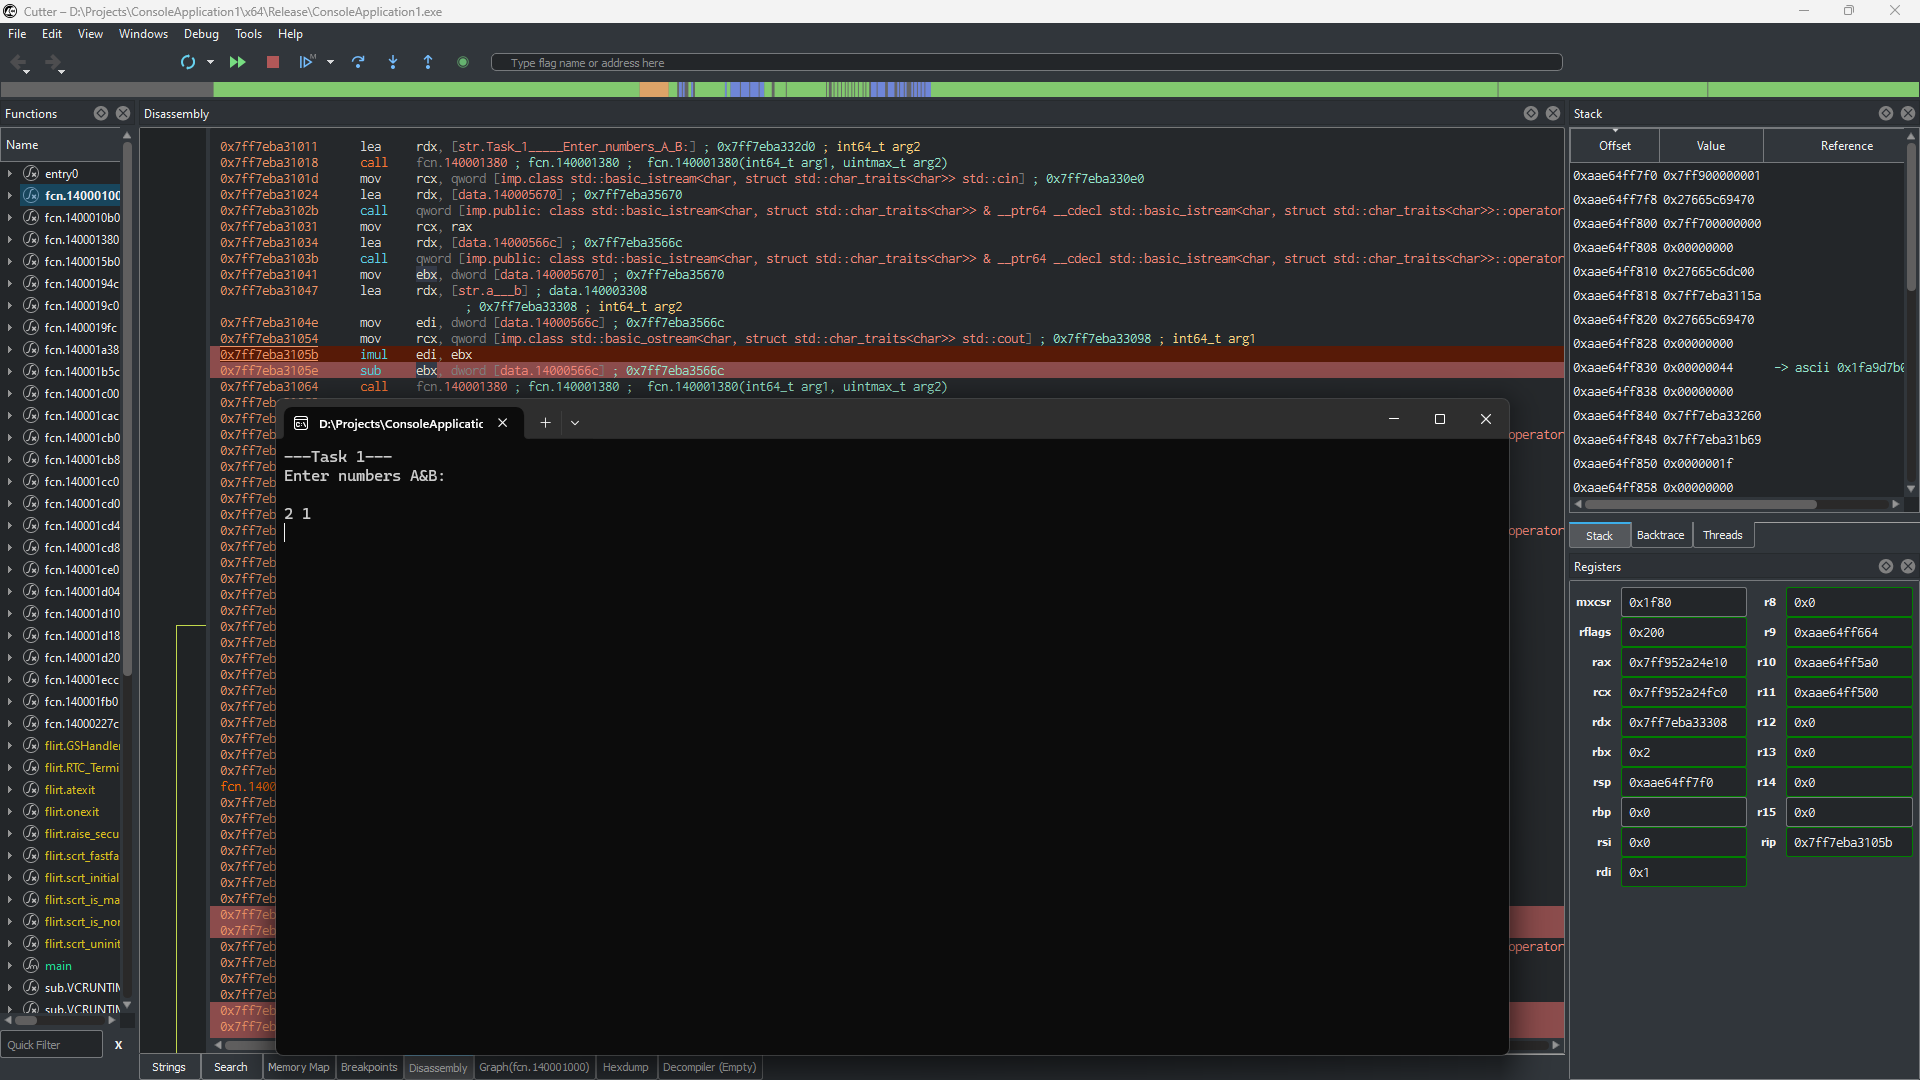
\includegraphics[width=1\linewidth]{Prt sc/1_1.png}  
        \end{minipage}
    \end{figure}
    \begin{figure}[h!]
        \begin{minipage}[h]{1\linewidth}
            \centering
            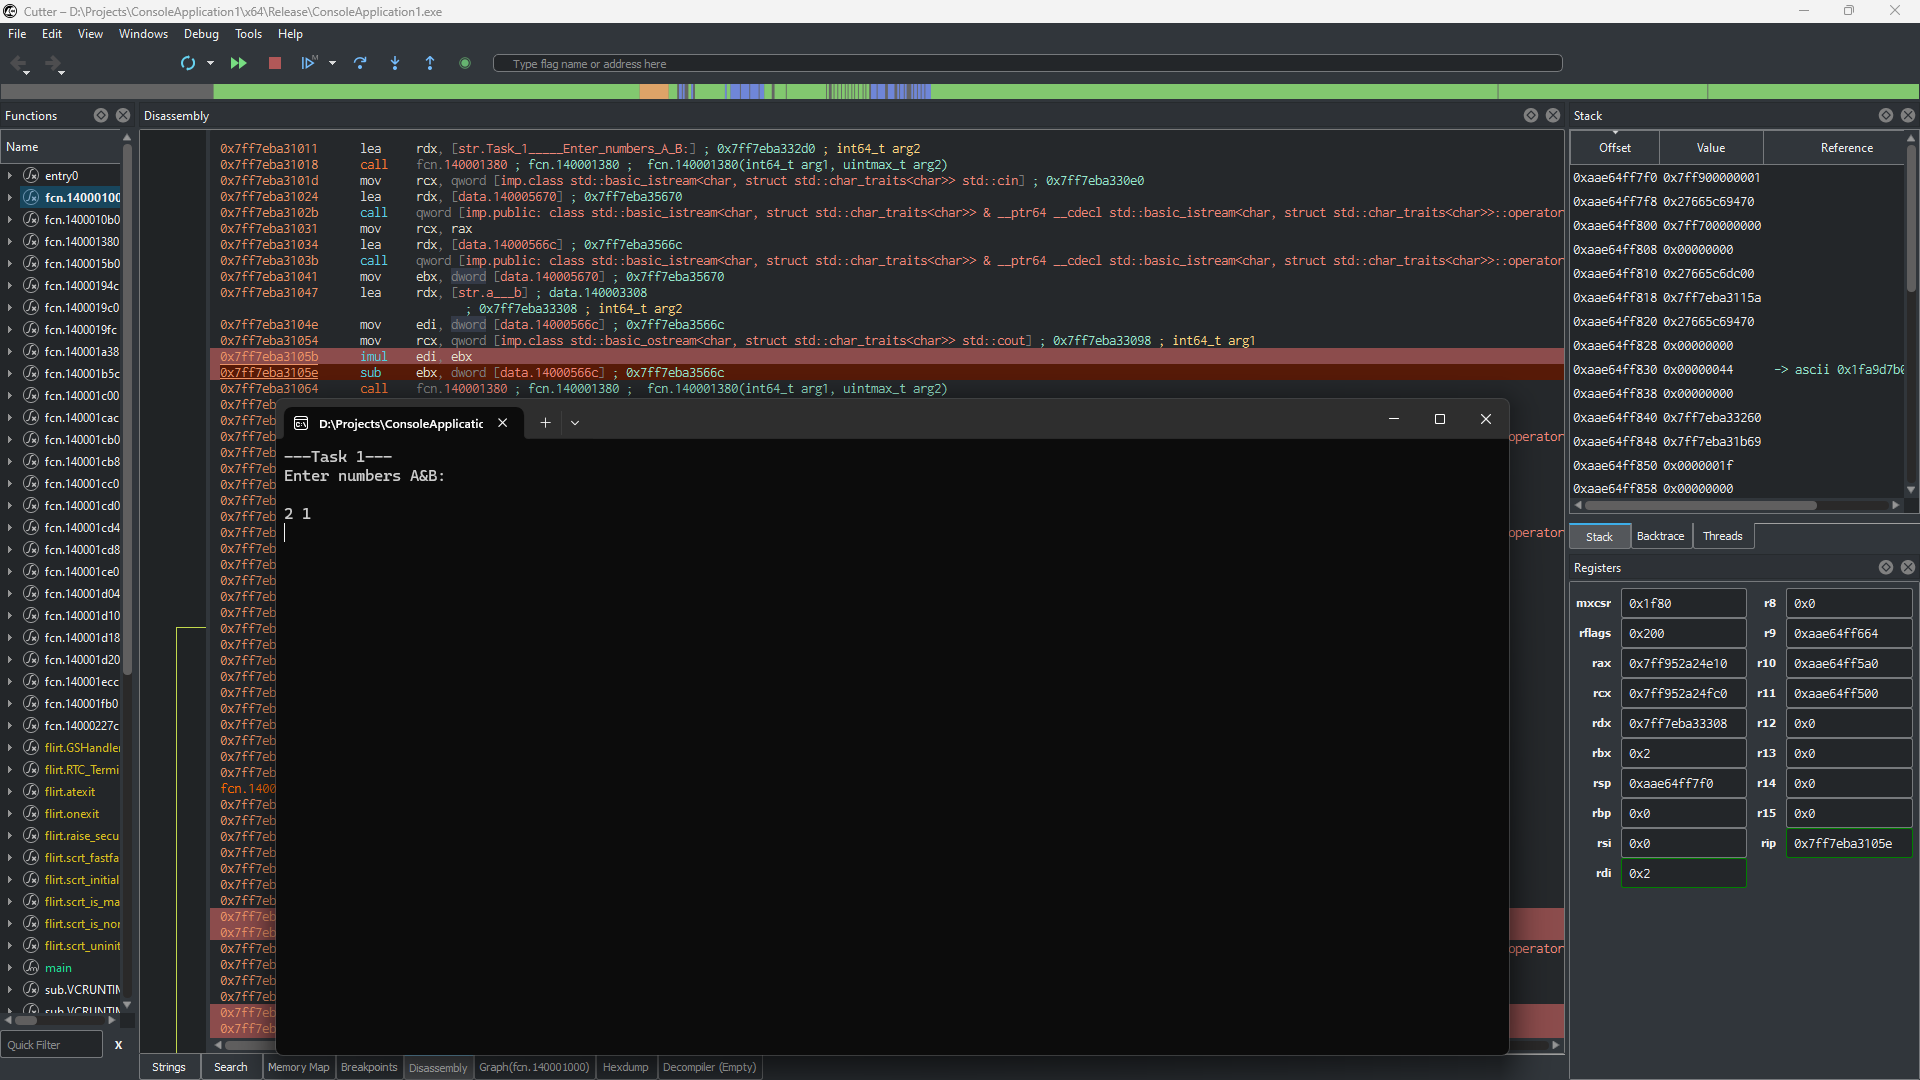
\includegraphics[width=1\linewidth]{Prt sc/1_2.png}  
        \end{minipage}
    \end{figure}

\newpage
    \begin{center}
        \Large{Task \RomanNumeralCaps{2}}
    \end{center}
    \begin{figure}[h!]
        \begin{minipage}[h]{1\linewidth}
            \centering
            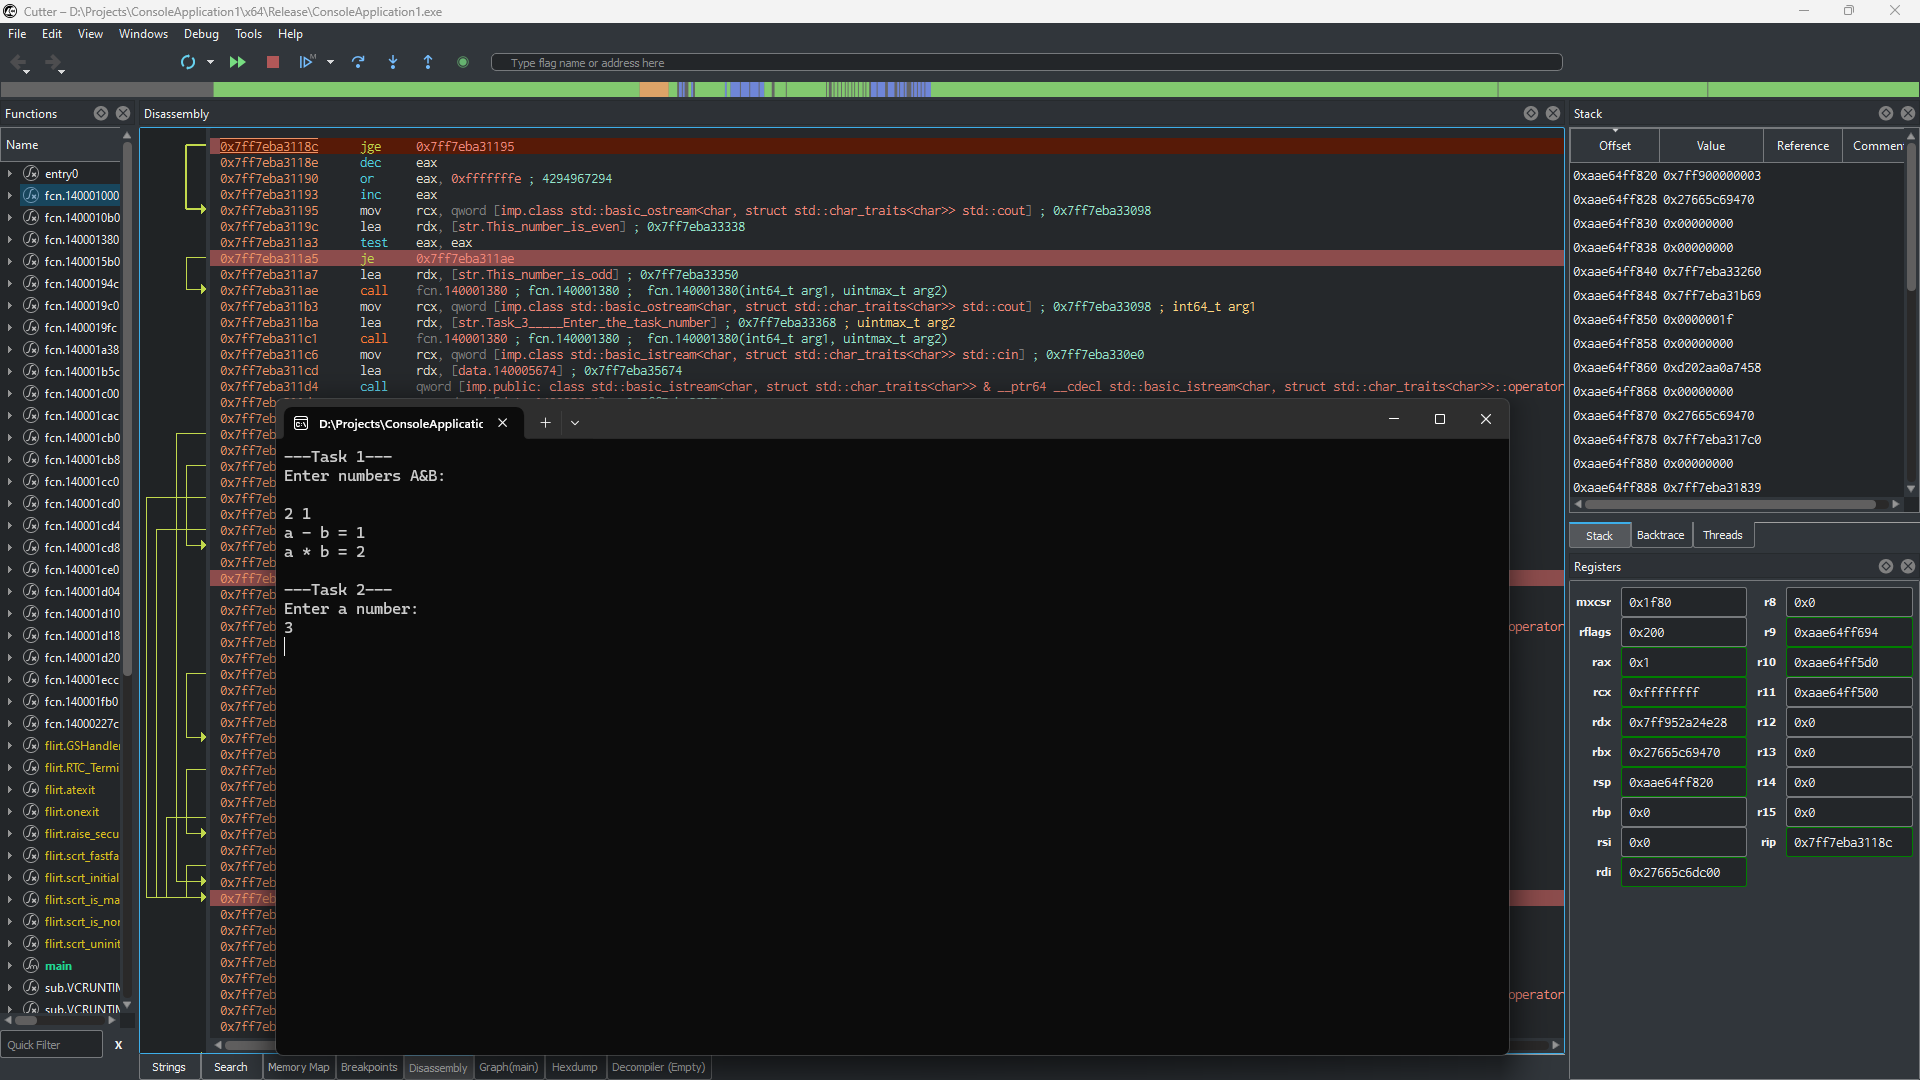
\includegraphics[width=1\linewidth]{Prt sc/2_1.png}  
        \end{minipage}
    \end{figure}
    \begin{figure}[h!]
        \begin{minipage}[h]{1\linewidth}
            \centering
            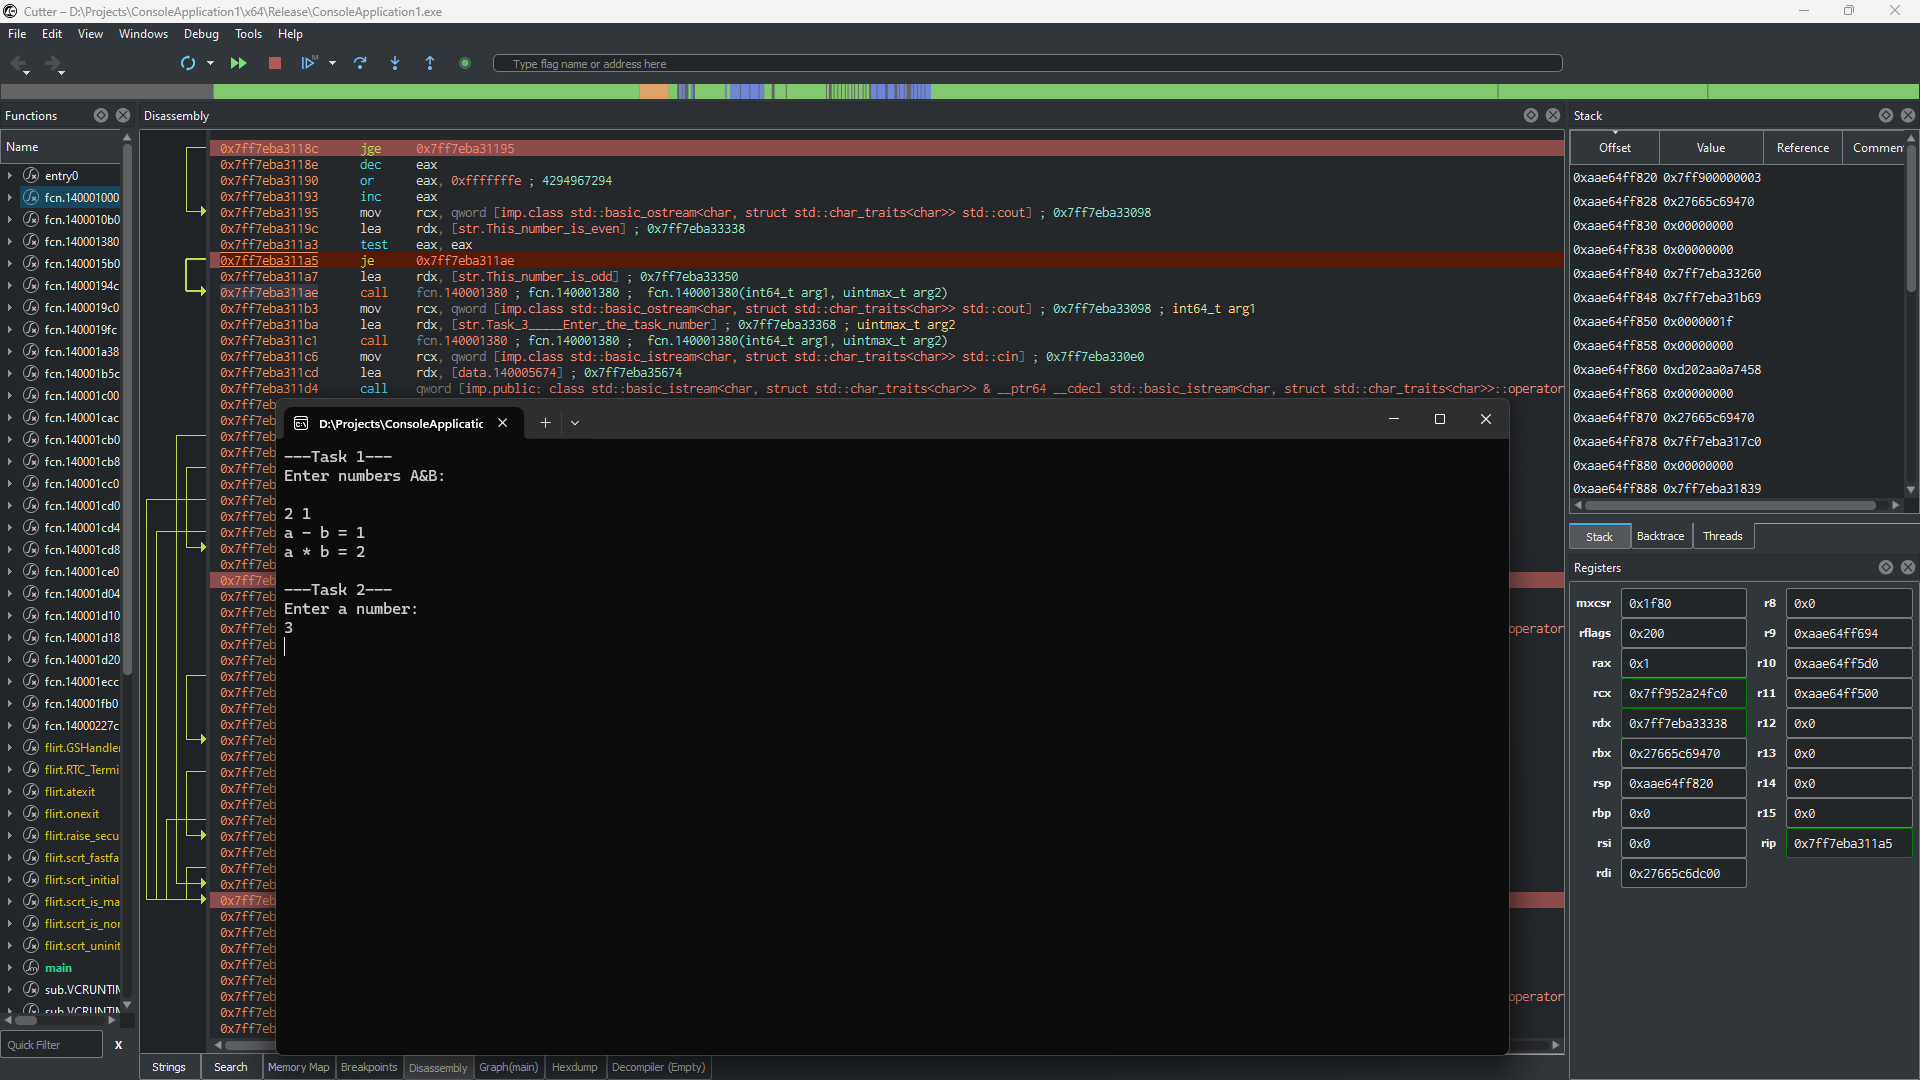
\includegraphics[width=1\linewidth]{Prt sc/2_2.png}  
        \end{minipage}
    \end{figure}

\newpage
    \begin{center}
        \Large{Task \RomanNumeralCaps{3}}
    \end{center}
    \begin{figure}[h!]
        \begin{minipage}[h]{1\linewidth}
            \centering
            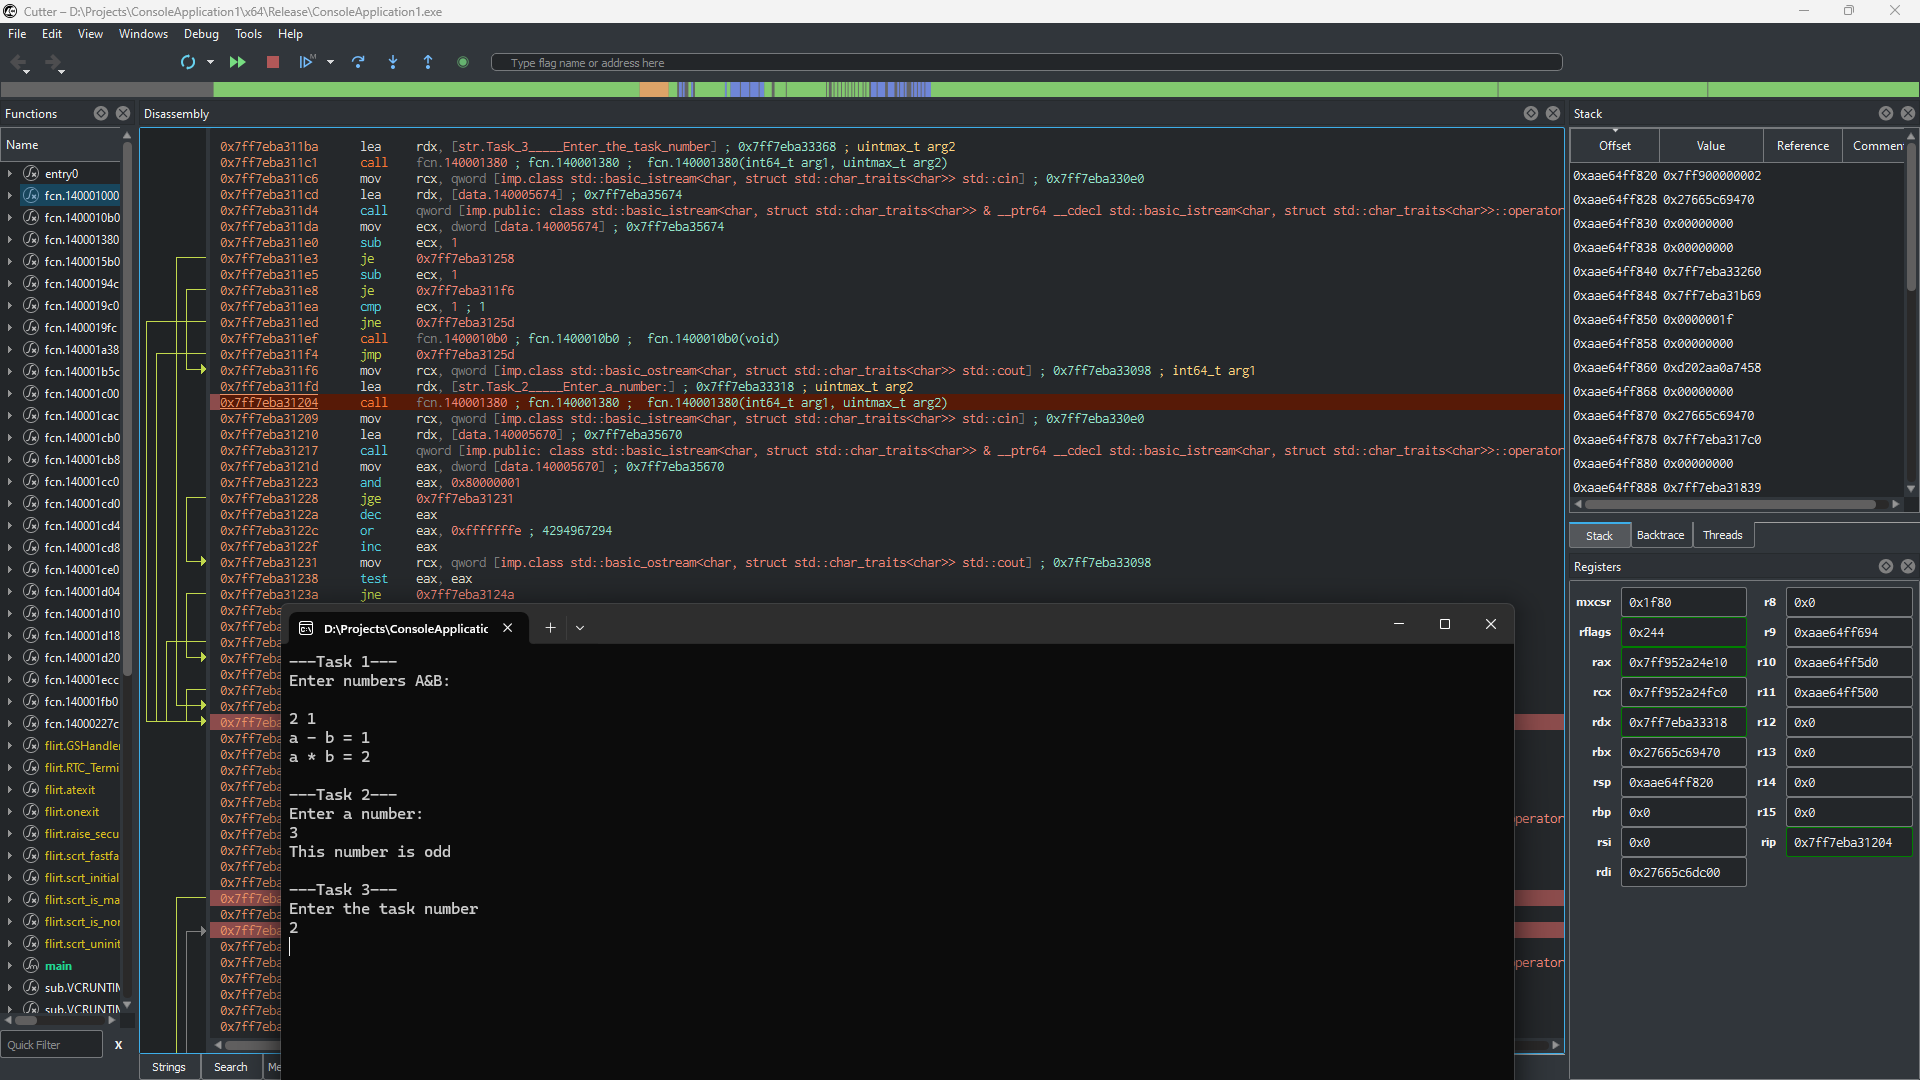
\includegraphics[width=1\linewidth]{Prt sc/3_1.png}  
        \end{minipage}
    \end{figure}
    \begin{center}
        \Large{Task \RomanNumeralCaps{4}}
    \end{center}
    \begin{figure}[h!]
        \begin{minipage}[h]{1\linewidth}
            \centering
            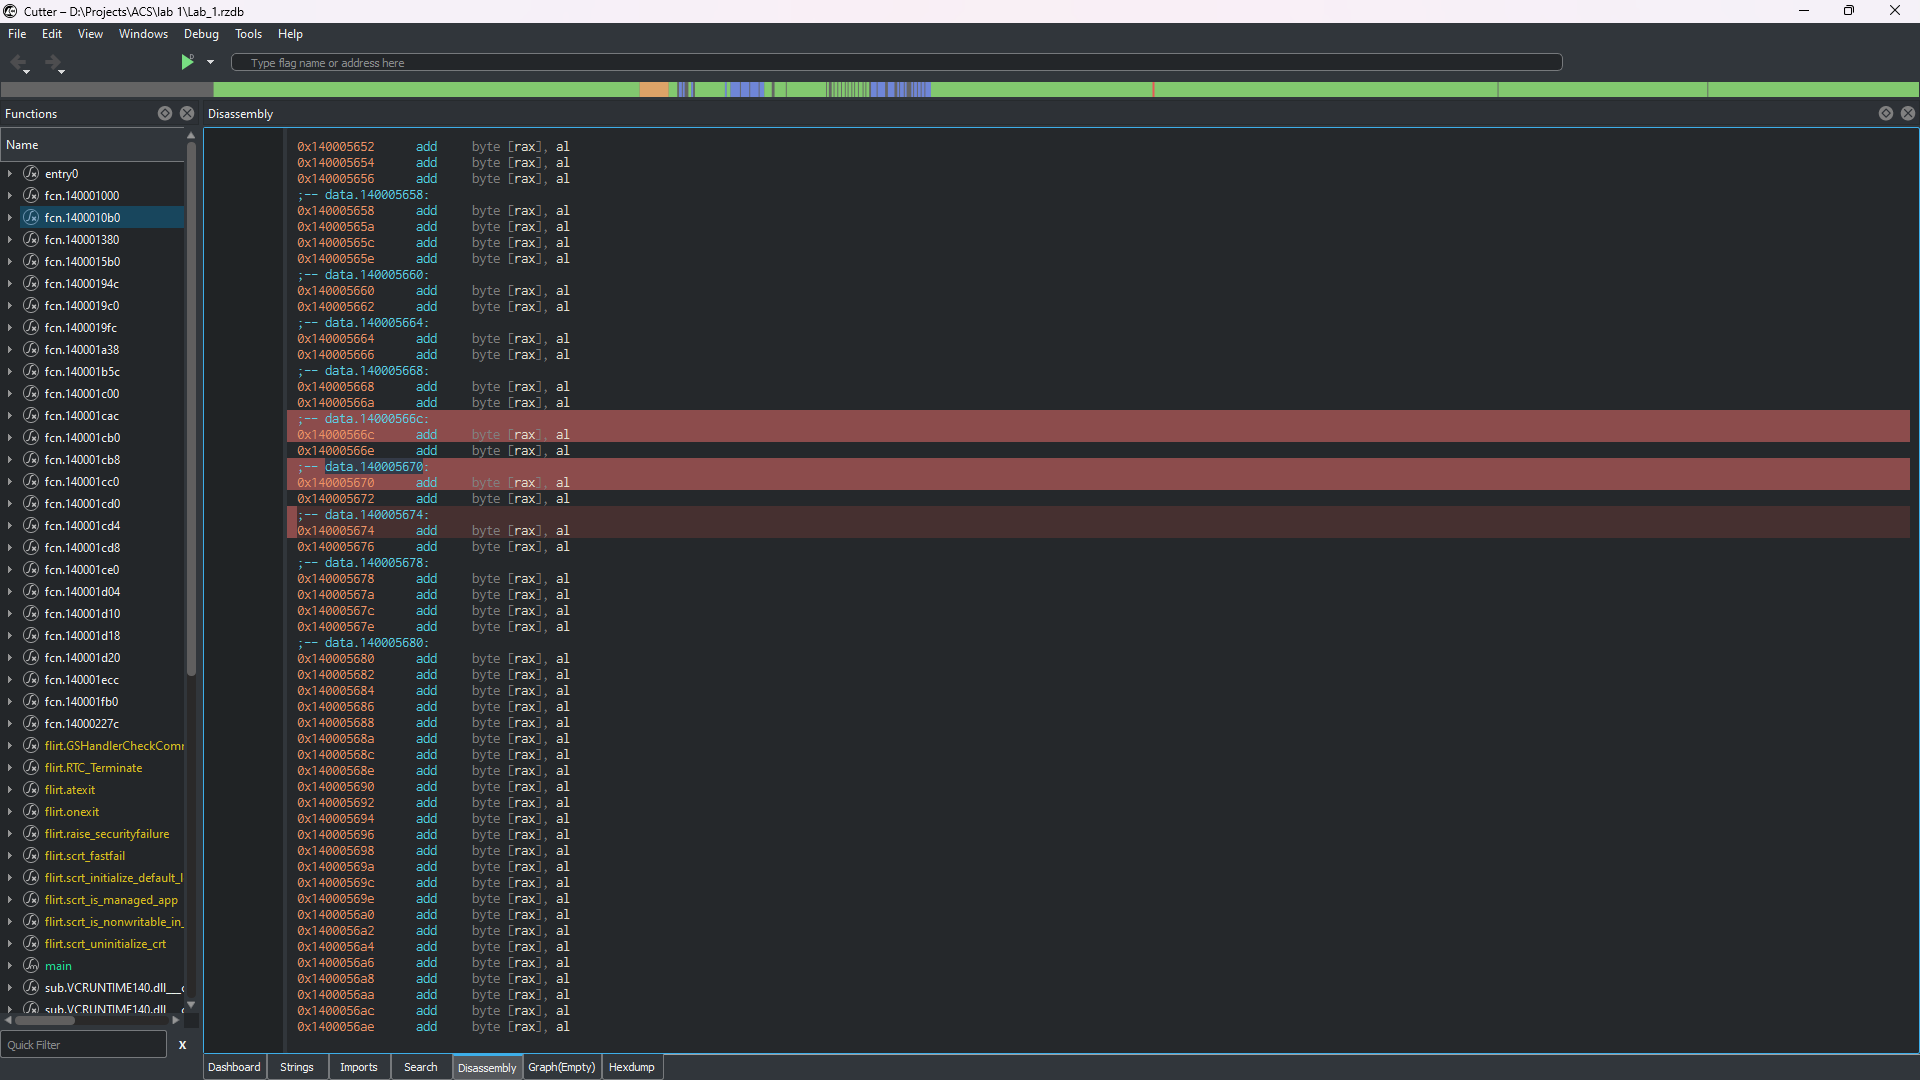
\includegraphics[width=1\linewidth]{Prt sc/4_0.png}  
        \end{minipage}
    \end{figure}

\newpage
    \begin{figure}[h!]
        \begin{minipage}[h]{1\linewidth}
            \centering
            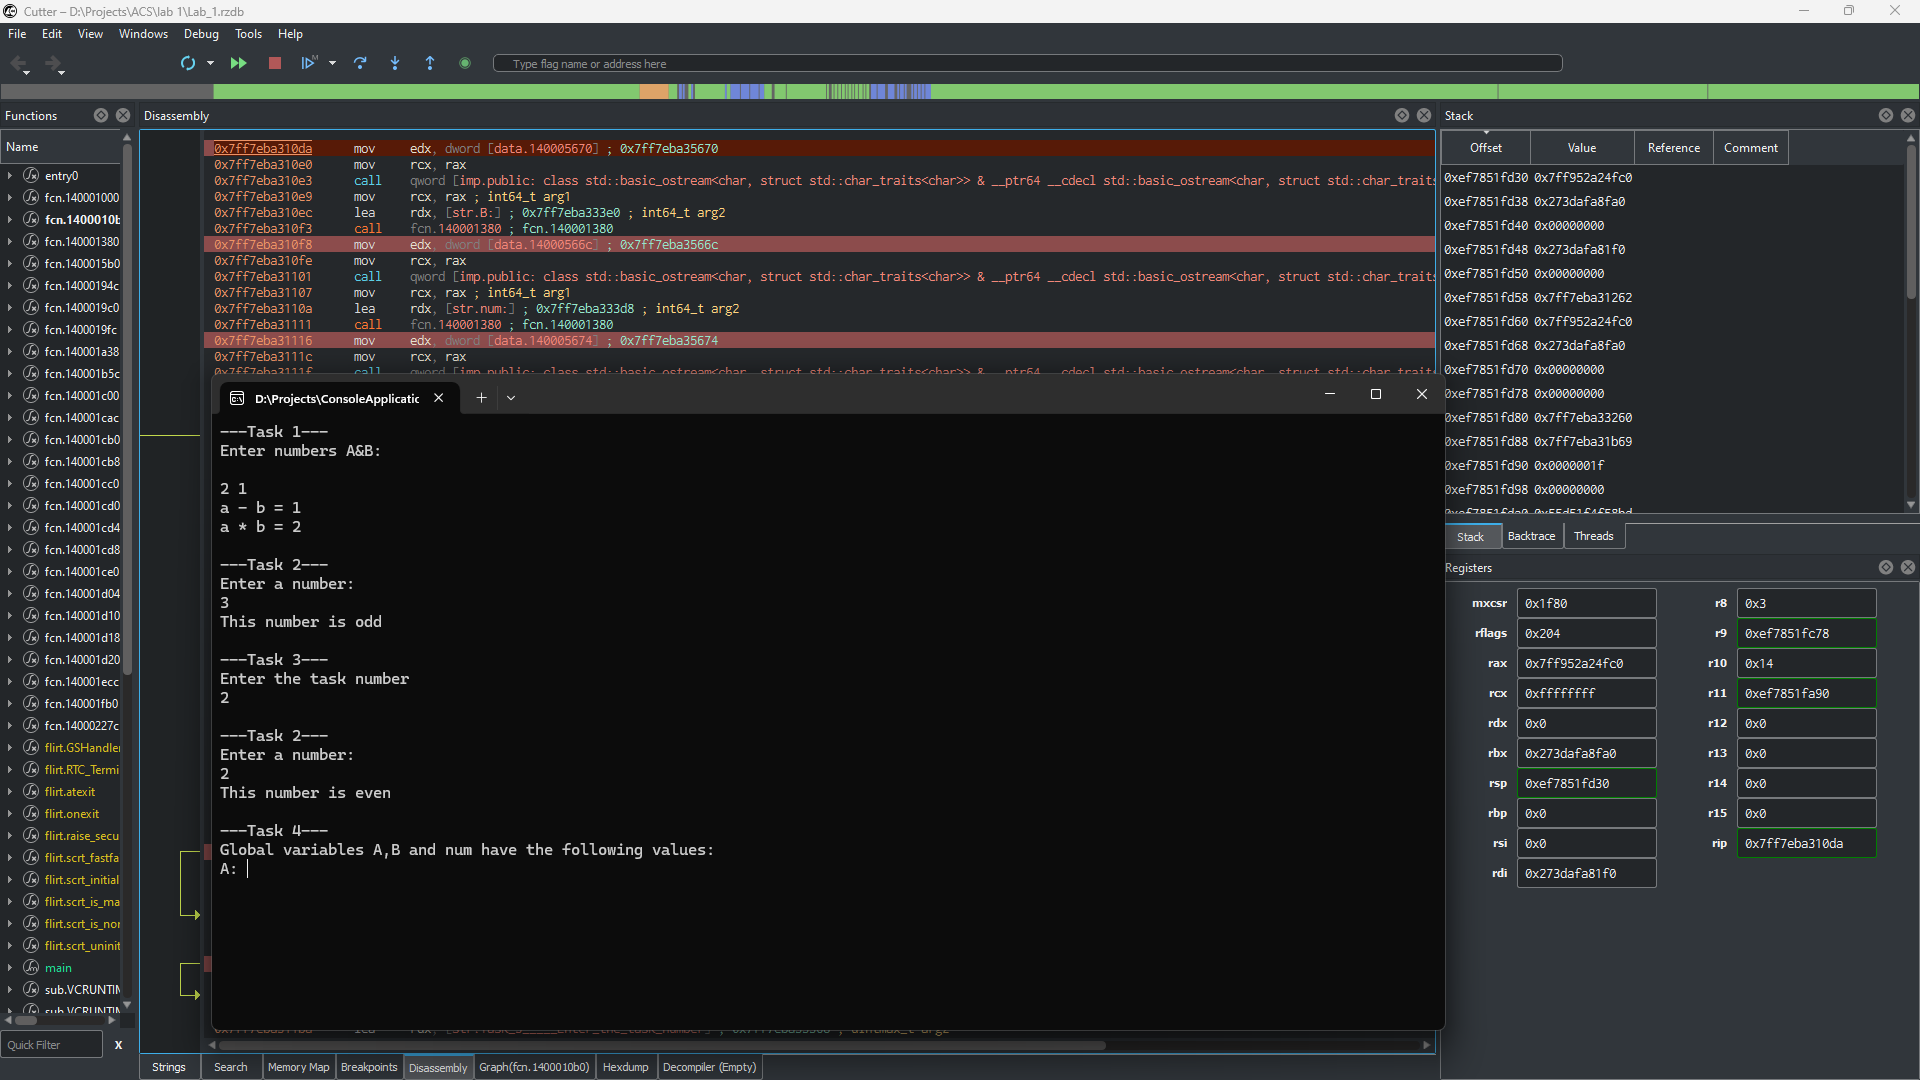
\includegraphics[width=1\linewidth]{Prt sc/4_1.png}  
        \end{minipage}
    \end{figure}
    \begin{figure}[h!]
        \begin{minipage}[h]{1\linewidth}
            \centering
            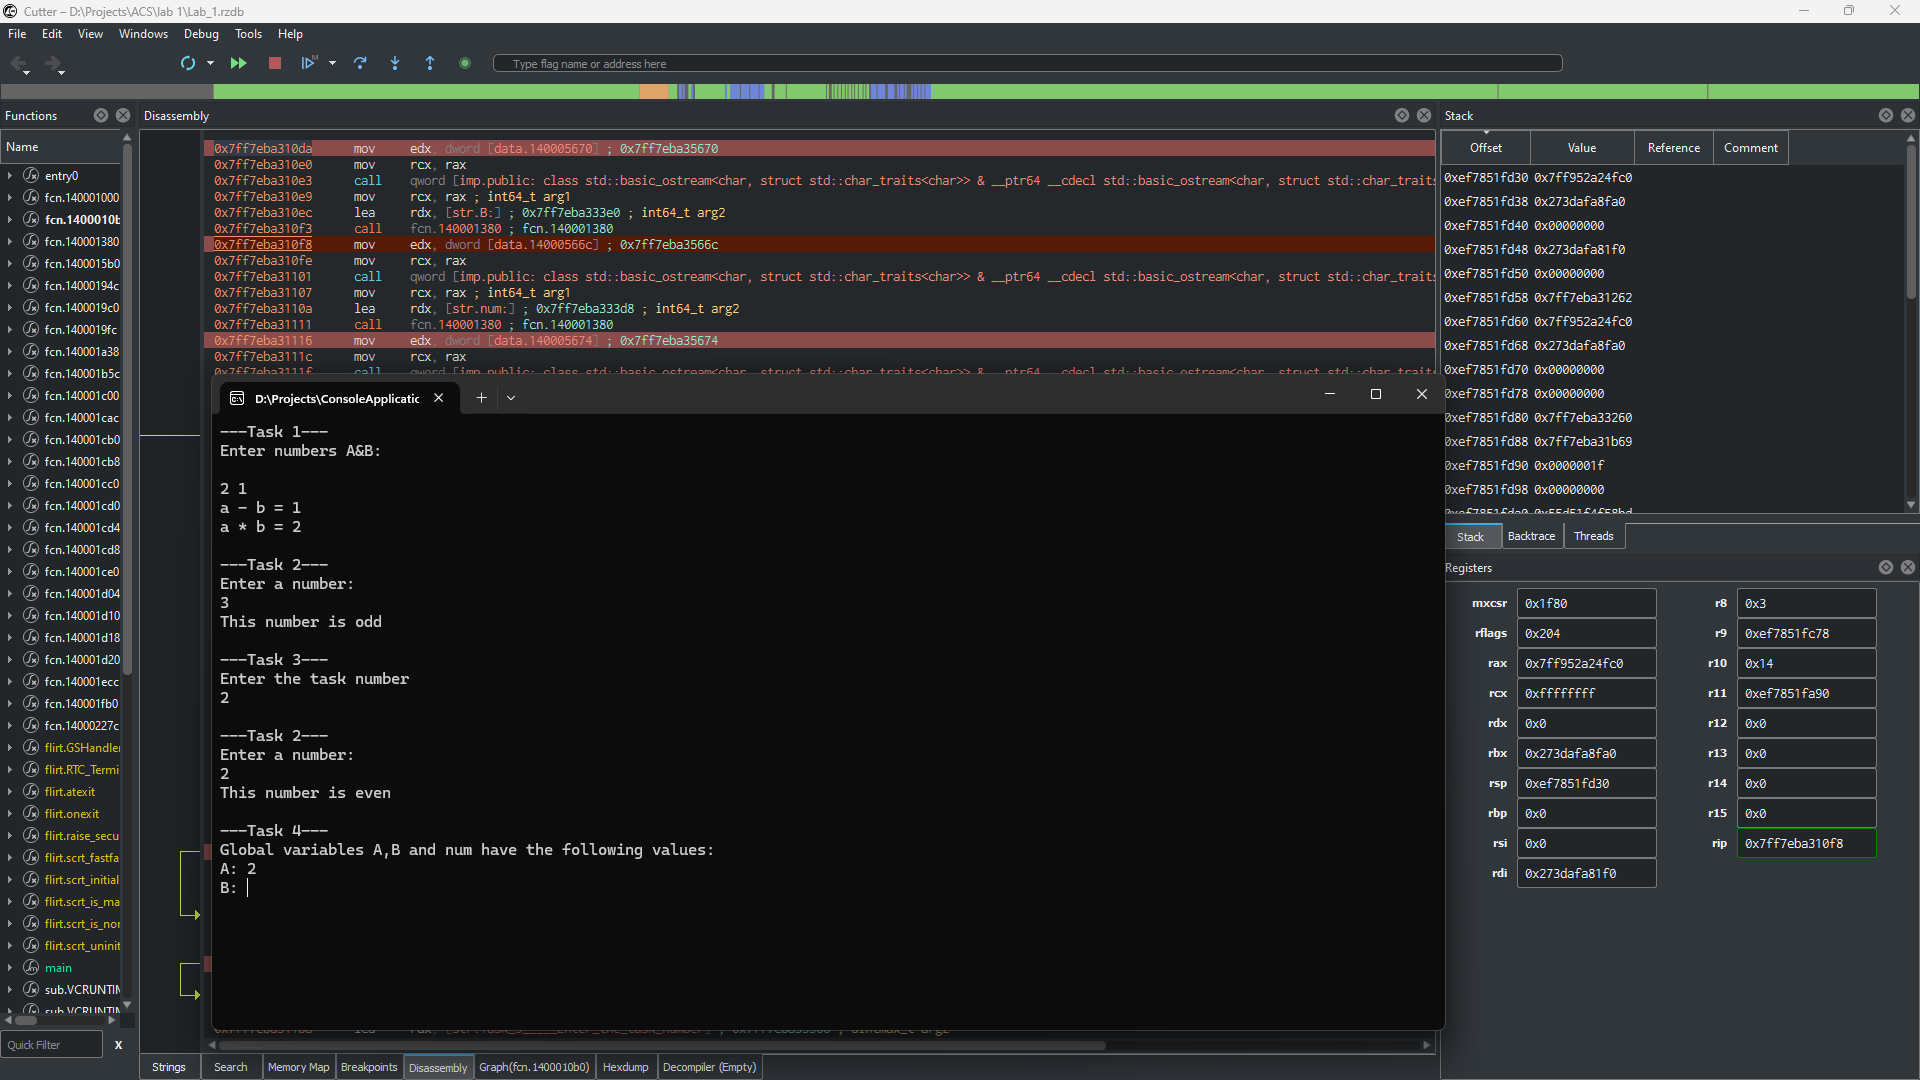
\includegraphics[width=1\linewidth]{Prt sc/4_2.png}  
        \end{minipage}
    \end{figure}

\newpage
    \begin{figure}[h!]
        \begin{minipage}[h]{1\linewidth}
            \centering
            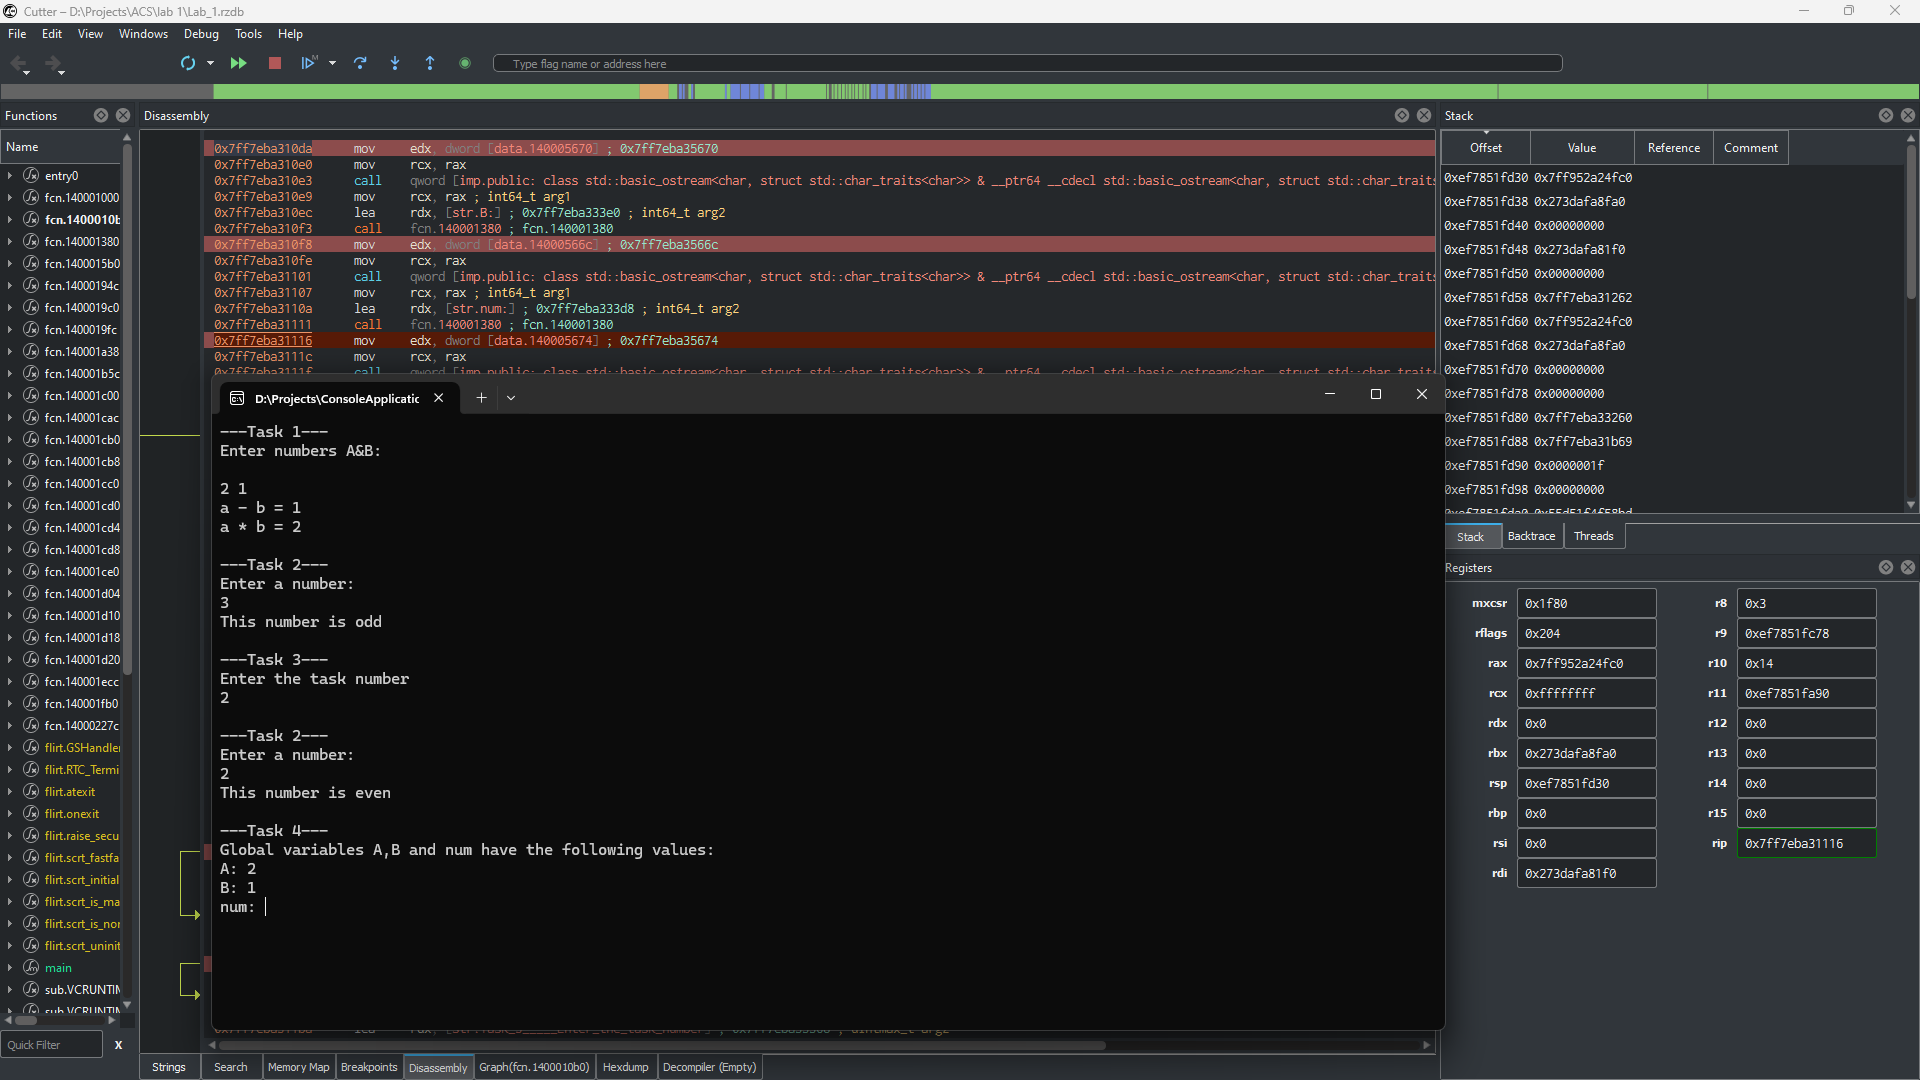
\includegraphics[width=1\linewidth]{Prt sc/4_3.png}  
        \end{minipage}
    \end{figure}
    \begin{center}
        \Large{Task \RomanNumeralCaps{5}}
    \end{center}
    \begin{figure}[h!]
        \begin{minipage}[h]{1\linewidth}
            \centering
            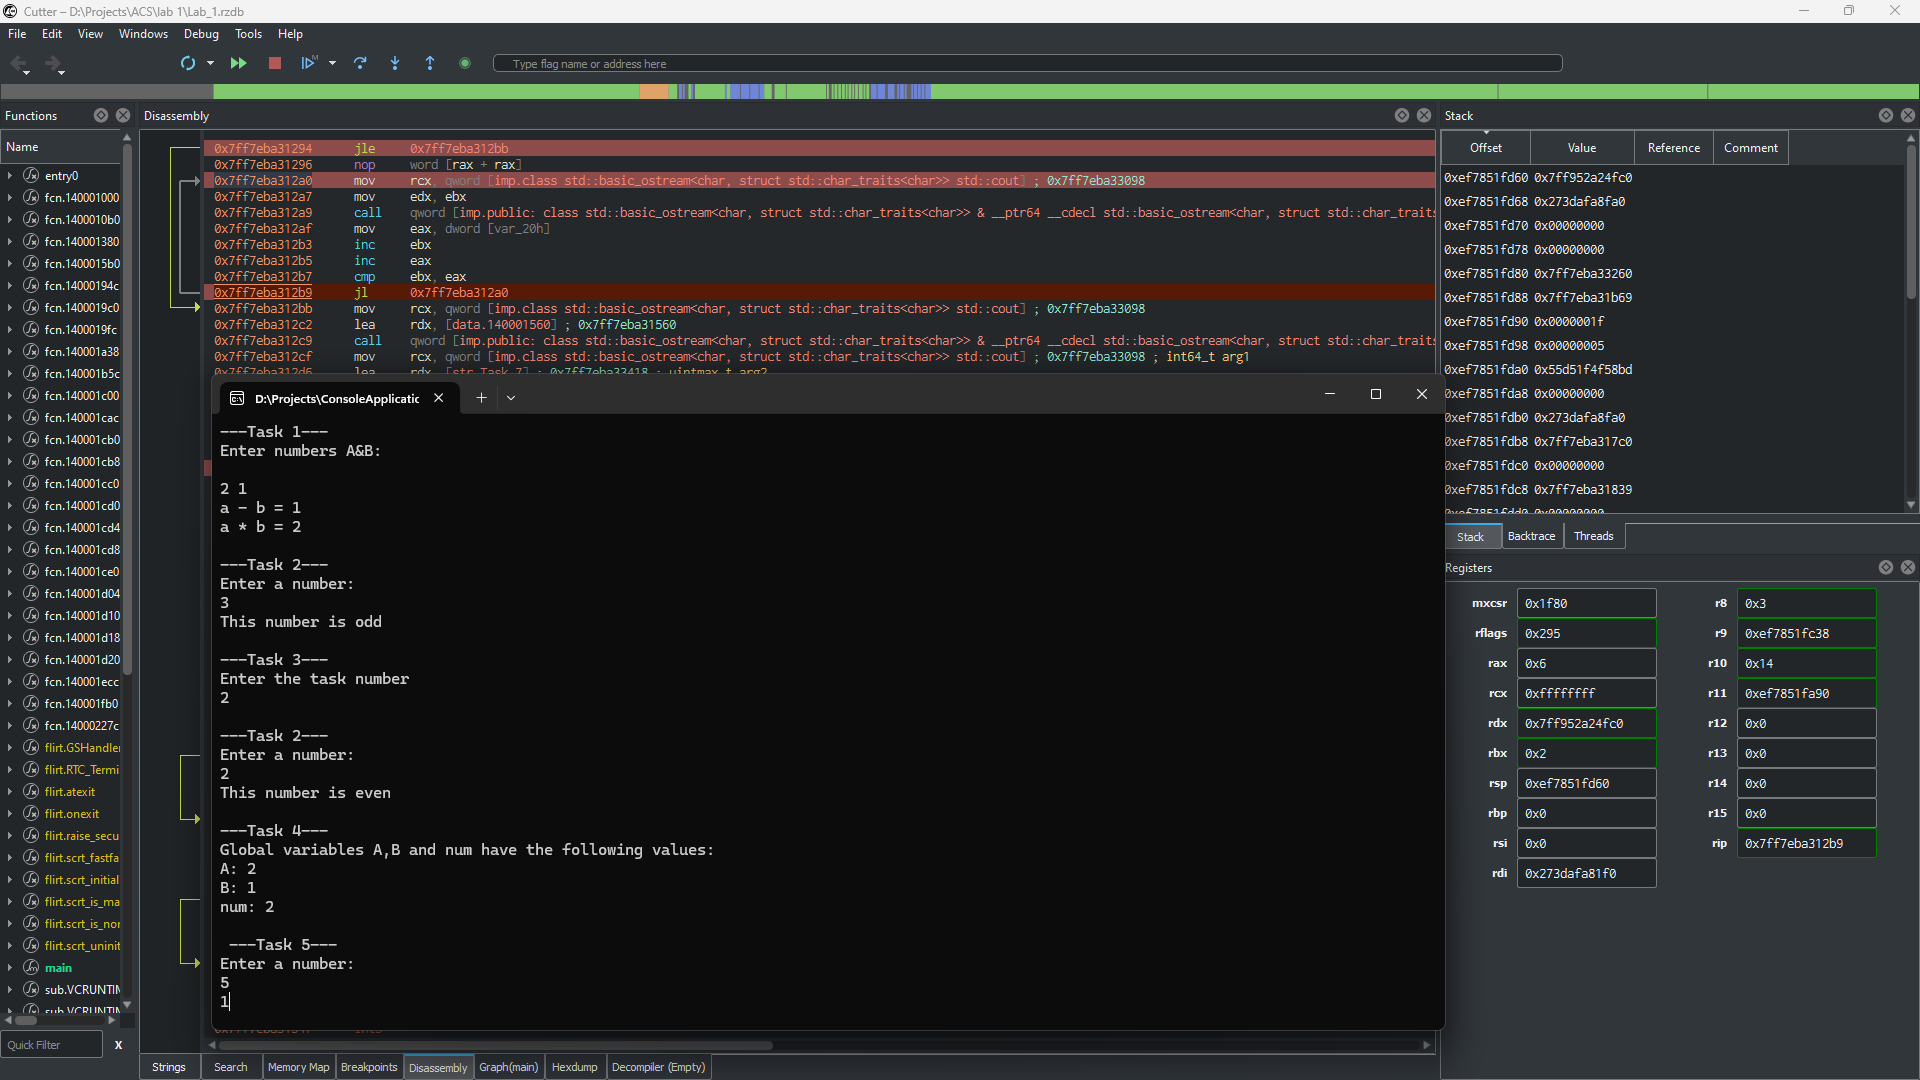
\includegraphics[width=1\linewidth]{Prt sc/5_1.png}  
        \end{minipage}
    \end{figure}

\newpage
    \begin{center}
        \Large{Task \RomanNumeralCaps{6}}
    \end{center}
    \begin{figure}[h!]
        \begin{minipage}[h]{1\linewidth}
            \centering
            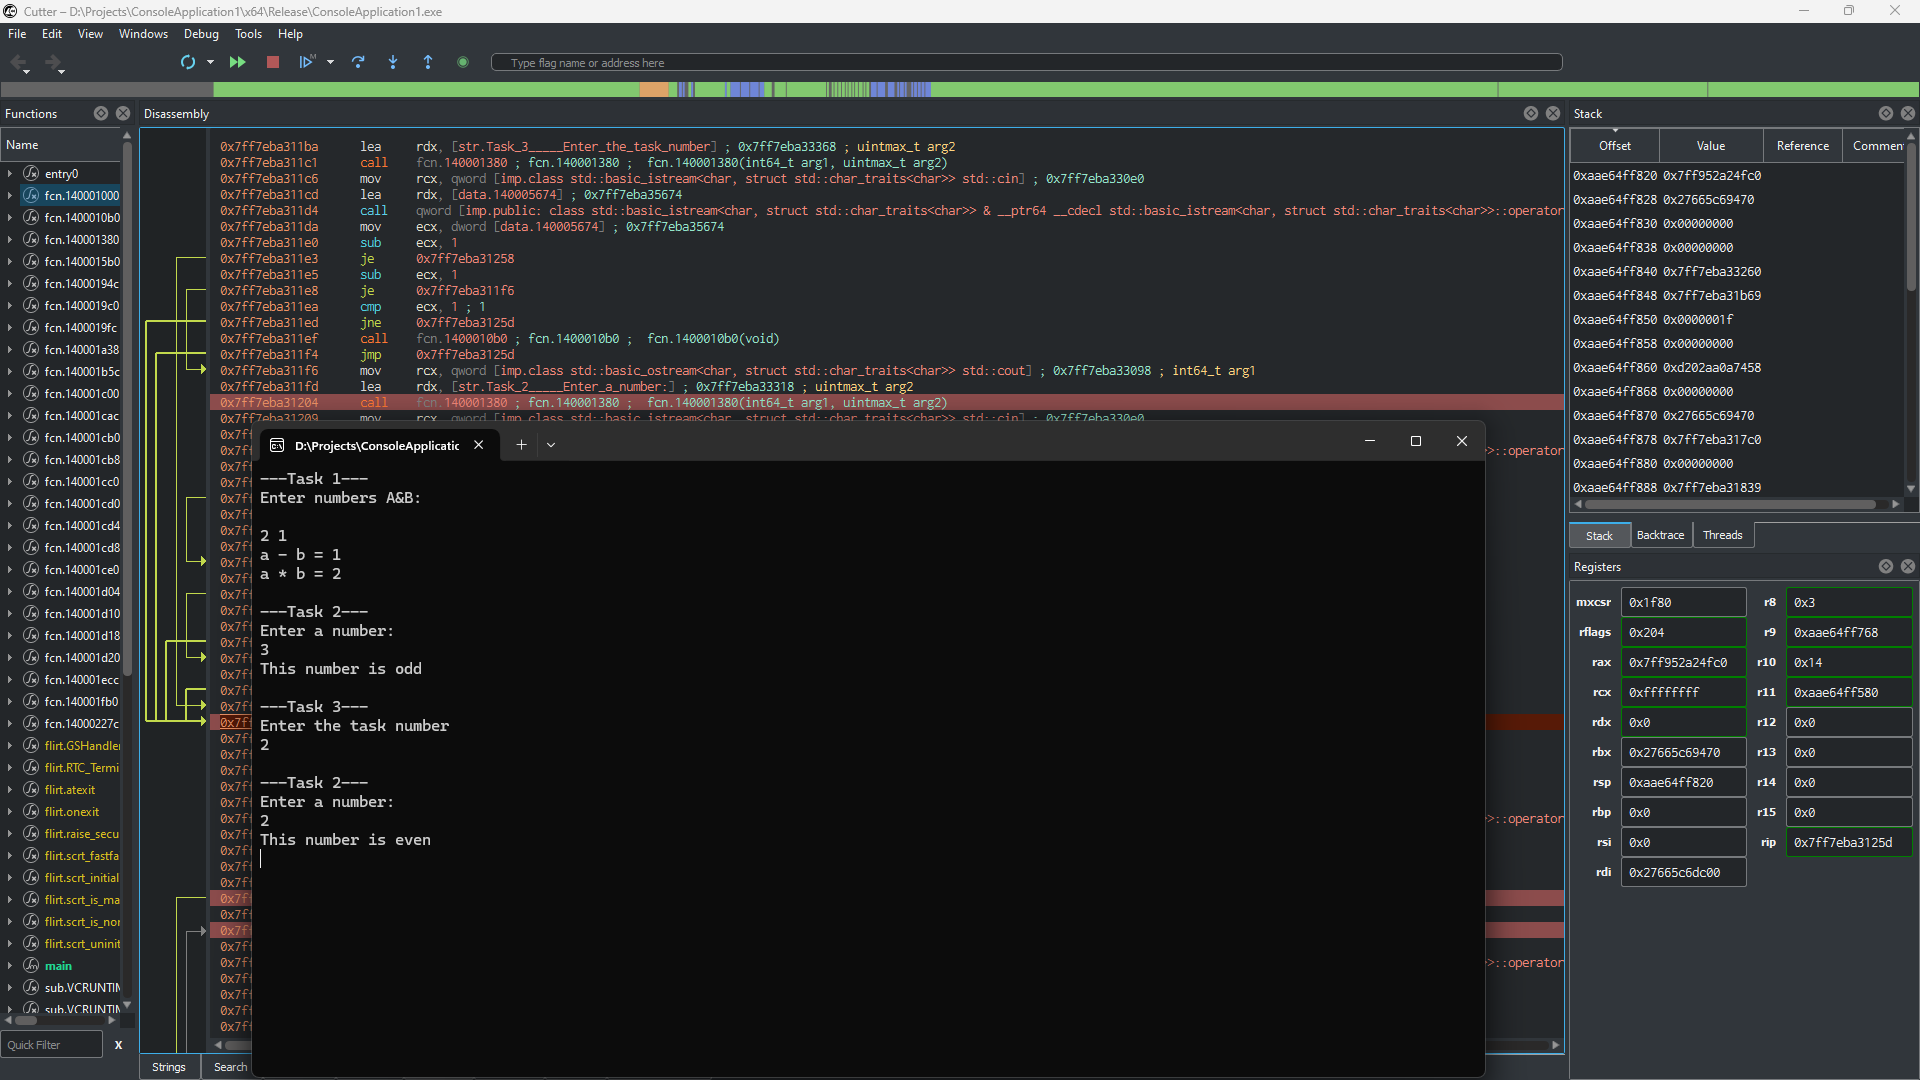
\includegraphics[width=1\linewidth]{Prt sc/6_1.png}  
        \end{minipage}
    \end{figure}
    \begin{center}
        \Large{Task \RomanNumeralCaps{7}}
    \end{center}
    \begin{figure}[h!]
        \begin{minipage}[h]{1\linewidth}
            \centering
            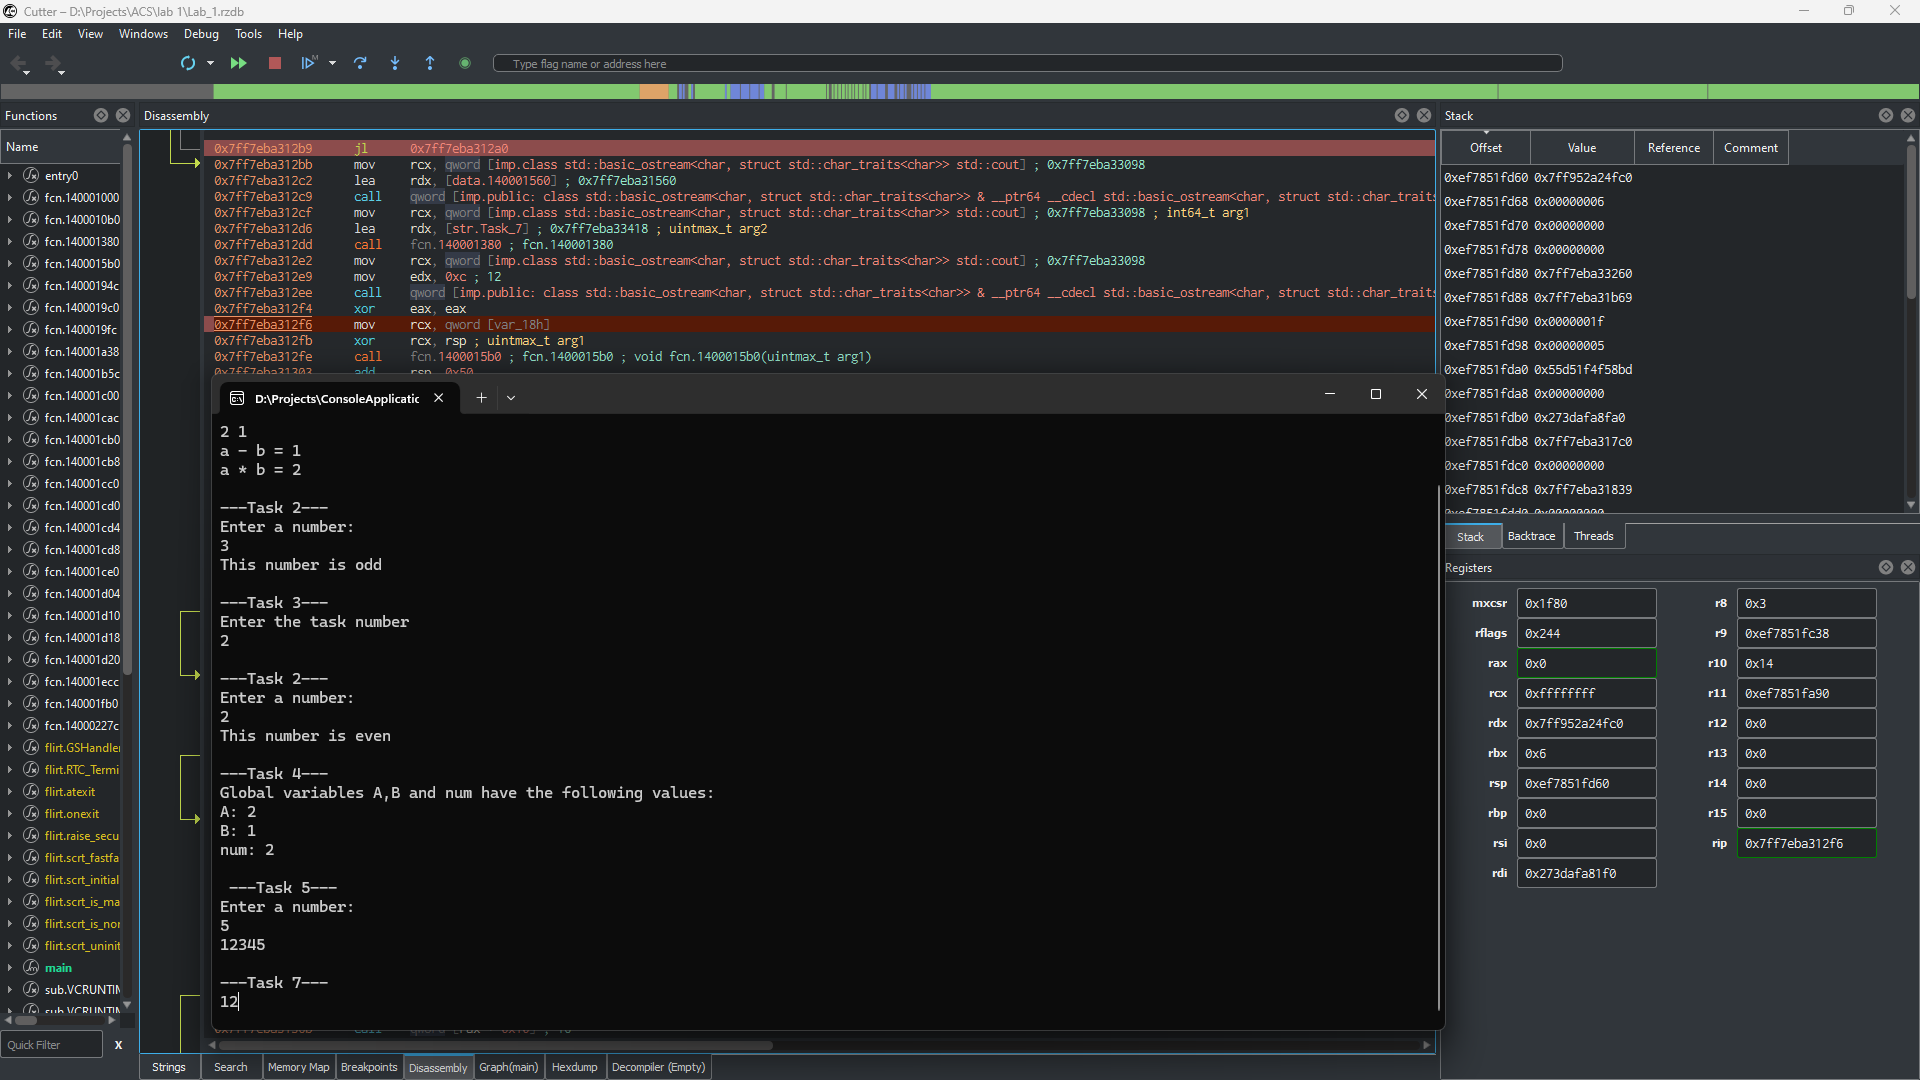
\includegraphics[width=1\linewidth]{Prt sc/7_1.png}  
        \end{minipage}
    \end{figure}

\end{document}